\section{Reaching New Heights: Finding the Peak Response Angle!}

\begin{tcolorbox}[colback=gray!10, colframe=black, title=E9B06]
What is the elevation angle of peak response in the antenna radiation pattern shown in Figure E9-2?
\begin{enumerate}[label=\Alph*.]
    \item 45 degrees
    \item 75 degrees
    \item \textbf{7.5 degrees}
    \item 25 degrees
\end{enumerate} \end{tcolorbox}

\subsubsection{Related Concepts}
To understand the concept of antenna radiation patterns and the corresponding elevation angles, we need to consider the following:

1. \textbf{Antenna Radiation Patterns:}: They describe how the radiated power of an antenna varies with direction. These patterns are typically depicted in polar or Cartesian coordinates.
2. \textbf{Elevation Angle:}: This is the angle between the horizontal plane and the direction of the antenna's peak response. In many applications, it helps in determining the optimal positioning of antennas for communication purposes.

In the given question, we are required to identify the elevation angle where the radiation pattern's peak response occurs. This angle is crucial for optimizing the coverage area and ensuring effective communication.

\subsubsection{Calculation Steps}
If calculations are necessary, we typically analyze the geometry of the antenna's radiation pattern. However, based on the given options and common patterns associated with antennas, the correct peak response usually correlates with lower angles for directional antennas.

\subsubsection{Diagram}
Assuming a typical scenario where an antenna's elevation pattern is depicted, we can briefly outline how a diagram could be illustrated using TikZ:

\begin{center}
\begin{tikzpicture}
    \draw[->] (0,0) -- (2,0) node[right] {0 degrees};
    \draw[->] (0,0) -- (0,2) node[above] {Power};
    \draw[domain=0:90,smooth,variable=\x,blue] plot ({\x},{sin(\x)}) node[right] {Radiation Pattern};
    \draw[dashed] (0:0) -- (0.5,0.5) node[above right] {7.5 degrees};
\end{tikzpicture}
\end{center}

In this diagram, the y-axis represents the power level, and the x-axis represents the elevation angle. The peak shown corresponds to the expected response value at its maximum, which, as per the provided choices, is \textbf{7.5 degrees}. 

Thus, we conclude that the correct answer to the question posed is \textbf{C: 7.5 degrees:}. 
